% =====================================================================
%  Cargo-to-Door: Autonomous Last-Meter Delivery for Vertical Cities
%  Project Report
%  Authors: Yusuf Savas, Rumeysa Akgun Ileri, Dicle Naz Ozdemir
%  Build:  pdflatex report.tex   (run twice for ToC/LoF/LoT)
% =====================================================================
\documentclass[11pt,a4paper]{report}

% ---- Encoding & fonts -------------------------------------------------
\usepackage[utf8]{inputenc}
\usepackage[T1]{fontenc}
\usepackage{lmodern}
\usepackage{microtype}

% ---- Math -------------------------------------------------------------
\usepackage{amsmath}

% ---- Layout -----------------------------------------------------------
\usepackage[a4paper,margin=1in]{geometry}
\usepackage{setspace}
\onehalfspacing
\usepackage{parskip}
\usepackage{titlesec}
\usepackage{fancyhdr}
\setlength{\headheight}{14pt}
\pagestyle{fancy}
\fancyhf{}
\fancyhead[L]{\nouppercase{\leftmark}}
\fancyhead[R]{\thepage}
\renewcommand{\headrulewidth}{0.4pt}

% ---- Graphics & figures ----------------------------------------------
\usepackage{graphicx}
\graphicspath{{images/}}
\usepackage{float}
\usepackage{caption}
\usepackage{subcaption}

% ---- Tables -----------------------------------------------------------
\usepackage{booktabs}
\usepackage{tabularx}
\usepackage{array}
\usepackage{longtable}
\newcolumntype{L}[1]{>{\raggedright\arraybackslash}p{#1}}

% ---- Lists & misc -----------------------------------------------------
\usepackage{enumitem}
\setlist{itemsep=2pt,topsep=2pt}
\usepackage{xcolor}

% ---- Hyperlinks (load last) ------------------------------------------
\usepackage[colorlinks=true,
            linkcolor=black,
            citecolor=black,
            urlcolor=blue!60!black,
            pdftitle={Cargo-to-Door: Autonomous Last-Meter Delivery for Vertical Cities},
            pdfauthor={Yusuf Savas, Rumeysa Akgun Ileri, Dicle Naz Ozdemir}]{hyperref}

% ---- Title metadata ---------------------------------------------------
\title{\Huge \textbf{Cargo-to-Door} \\[0.4em]
       \LARGE Autonomous Last-Meter Delivery for Vertical Cities}
\author{Yusuf Sava\c{s} \and Rumeysa Akg\"un \.Ileri \and Dicle Naz \"Ozdemir}
\date{\today}

% =====================================================================
\begin{document}

% ---------------------------------------------------------------------
%  TITLE PAGE
% ---------------------------------------------------------------------
\begin{titlepage}
    \centering
    \vspace*{2.5cm}
    {\Huge\bfseries Cargo-to-Door\par}
    \vspace{0.6cm}
    {\LARGE Autonomous Last-Meter Delivery\\[0.2em] for Vertical Cities\par}
    \vspace{1.5cm}
    {\large Project Report\par}
    \vfill
    {\large
        Yusuf Sava\c{s}\\[0.2em]
        Rumeysa Akg\"un \.Ileri\\[0.2em]
        Dicle Naz \"Ozdemir\\
    }
    \vfill
    {\large \today\par}
\end{titlepage}

% ---------------------------------------------------------------------
%  ABSTRACT
% ---------------------------------------------------------------------
\chapter*{Abstract}
\addcontentsline{toc}{chapter}{Abstract}

The ``last meter'' of urban package delivery---the path from a building's
lobby to a resident's actual door---remains a manual, slow, and unreliable
bottleneck that drives roughly 30--50\% of total e-commerce logistics cost
and is amplified by porch piracy, failed deliveries, and the vertical
density of modern cities. This report presents \textbf{Cargo-to-Door}, a
twin-track autonomous logistics infrastructure that closes this gap. For
new high-rises, a centralized rooftop \emph{Flight Deck} receives
winch-dropped parcels from hovering drones into an aerodynamic catchment
funnel, after which gravity chutes, motorized roller conveyors, mechanical
diverters, and a smart dumbwaiter route each parcel into a resident's
hallway smart locker. For historic and protected buildings that cannot
be torn open, a modular \emph{Exo-Logistics Spine} clipped to the facade
houses an intelligent self-contained elevator car that reaches through
retrofitted window-box lockers. Both tracks share a multi-modal ground
intake that handles sidewalk micro-rovers via precision robotic
handovers. The report covers motivation, a literature and state-of-the-art
survey, requirements, system architecture, design with implementation and
testing strategy, a 24-month phased roadmap with work packages, and the
commercialization and business model.

% ---------------------------------------------------------------------
%  FRONT MATTER LISTS
% ---------------------------------------------------------------------
\tableofcontents
\listoffigures
\listoftables

% =====================================================================
%  CHAPTER 1 - MOTIVATION & PROBLEM DEFINITION
% =====================================================================
\chapter{Motivation and Problem Definition}
\label{ch:motivation}

The goal of this project is to engineer a continuous, autonomous, and
weatherproof path from the sky---or the sidewalk---to a resident's
apartment door, simultaneously for newly constructed high-rise towers and
for historic buildings that must be preserved.

\section{The Broken Last Mile and the Missing Last Meter}

Last-mile logistics is the single most expensive link in the e-commerce
supply chain, accounting for an estimated 30--50\% of total logistics
cost, and the dominant contributor to urban congestion and tailpipe
emissions. Within that already-strained link sits a second, often
overlooked, problem: the \emph{last meter}. Even after a parcel reaches a
building's lobby, the trip up to the apartment door is performed
manually---by couriers riding crowded elevators, by neighbors holding the
door, or by residents who must come down to a lobby concierge. The
result is slow, unreliable, labor-intensive delivery; failed handoffs
trigger expensive returns, and unattended porch deliveries fuel theft
(``porch piracy'') and customer churn.

\section{Why Vertical Density Breaks Current Solutions}

The autonomous delivery wave---drones, sidewalk micro-rovers, and
in-building robots---was designed primarily for suburban or low-density
urban contexts and does not survive contact with vertical cities:
\begin{itemize}
    \item Drones cannot safely land on balconies due to wind shear,
          rotor downwash, and the absence of certified landing zones.
    \item Sidewalk micro-rovers cannot ride elevators or climb stairs,
          so they stop at the lobby.
    \item Human couriers cannot scale to towers with hundreds of
          apartments per stack without dominating the elevator network.
    \item Parcel-locker arrays force the resident to come down, which
          defeats the door-to-door promise.
\end{itemize}

\section{The Historic-Building Constraint}

A parallel constraint exists in the other half of the urban building
stock: protected and historic buildings cannot be torn open to install
new vertical infrastructure, and their masonry, electrical, and aesthetic
codes severely restrict facade modifications. Yet their residents demand
the same level of service as those in new smart-buildings. Any credible
solution must therefore offer both a \emph{new-build} integration and a
\emph{retrofit} variant that respects historic-preservation rules.

\section{Problem Statement}

Cargo-to-Door addresses the combined last-mile and last-meter problem in
vertical, dense, mixed-age cities by providing a single
building-integrated infrastructure that (i)~accepts multi-modal
deliveries from aerial drones, sidewalk rovers, and human couriers,
(ii)~transports parcels vertically inside the building without human
labor, and (iii)~deposits each parcel into a secure, authenticated
endpoint on the resident's own floor---all while remaining
weatherproof, low-noise, and structurally reversible for retrofit
deployments.

% =====================================================================
%  CHAPTER 2 - LITERATURE SURVEY
% =====================================================================
\chapter{Literature Survey}
\label{ch:literature}

This chapter reviews the academic literature on high-density autonomous
delivery, surveys the present industrial state of the art across seven
delivery archetypes, articulates the proposed twin-track Cargo-to-Door
solution and its innovation aspects, and enumerates the breakthrough
technologies the system depends on.

\section{Literature Review}
\label{sec:lit-review}

Recent research has begun to address the specific problems of
high-density and high-rise delivery, the wind environment around tall
buildings, and the optimization of drone infrastructure. Five
representative studies are summarized in Table~\ref{tab:lit-review}.

\begin{table}[H]
\centering
\caption{Representative academic literature on drone-based high-density delivery.}
\label{tab:lit-review}
\small
\begin{tabularx}{\linewidth}{L{4.0cm} L{2.8cm} L{2.8cm} X}
\toprule
\textbf{Study} & \textbf{Objective} & \textbf{Method} & \textbf{Findings} \\
\midrule
UAVs for High-Density Residential Delivery (2022) \cite{uav2022}
    & Holistic delivery in high-density residential areas
    & Facade integration and network control
    & Temperature-controlled facade parcel intake units and 3D urban models \\
\addlinespace
Drone High-Rise Aerial Delivery with Vertical Grid Screening (2023) \cite{grid2023}
    & Vertical grid-based delivery structures
    & Vertical grid screening and experimental testing
    & Optimized vertical approach and wind-protected intake stations \\
\addlinespace
Drones in last-mile delivery: a systematic literature review (2024) \cite{slr2024}
    & Synthesize research on logistics challenges and opportunities
    & Systematic literature review (SLR)
    & Identifies gaps in operational feasibility, regulation, and business-model sustainability \\
\addlinespace
Integrated Planning of Infrastructure and Drone Delivery Operations with Multiple Cycles (2025) \cite{integrated2025}
    & Multi-cycle infrastructure and operational integration
    & Mathematical optimization and energy modeling
    & Lower energy consumption, 29\% wider coverage area, smart routing \\
\addlinespace
Wind-Aware Service Provisioning for Multi-Package Drone Delivery (2025) \cite{wind2025}
    & Wind awareness in multi-package deliveries
    & Spatio-temporal DaaS model and genetic algorithms
    & Service sharing and composition, 10.1\% energy savings \\
\bottomrule
\end{tabularx}
\end{table}

The literature converges on two consistent conclusions. First, drones
\emph{can} reach high-rise residents reliably only when the building
itself participates---through facade intake units, vertical grid
screening, or wind-mitigation geometry. Second, the operational,
regulatory, and business-model dimensions of urban drone delivery are
still under-developed; piecemeal point solutions have not produced a
deployable system. Cargo-to-Door sits at the intersection of these two
findings by treating the building as a first-class element of the
delivery infrastructure.

\section{Past Solutions and the State of the Art}
\label{sec:sota}

The present industrial landscape contains seven recognizable archetypes
of autonomous or semi-autonomous urban delivery. Table~\ref{tab:sota}
summarizes their providers, strengths, and the limitations that motivate
Cargo-to-Door.

\begin{table}[H]
\centering
\caption{Industrial state of the art in urban autonomous delivery.}
\label{tab:sota}
\small
\begin{tabularx}{\linewidth}{L{3.0cm} L{3.4cm} X X}
\toprule
\textbf{Approach} & \textbf{Providers} & \textbf{Strengths} & \textbf{Limitations} \\
\midrule
Drone-to-doorstep
    & Wing, Zipline, Matternet, Amazon Prime Air, Manna, Flytrex, Meituan, Uber \& Manna
    & Bypasses ground congestion; fastest rural/suburban last-mile; ideal for urgent medical supplies.
    & Weather-sensitive; one parcel per flight; needs landing pad or winch; not vertical-city friendly. \\
\addlinespace
Heavy-duty cargo drones
    & Elroy Air, Volocopter, Dronamics
    & VTOL, no runway; high-speed middle-mile between regional hubs.
    & Cannot deliver to consumer doorsteps; strict airspace regulations; high energy. \\
\addlinespace
Sidewalk micro-rovers
    & Starship, Serve, Coco, Kiwibot, Yandex Rover, Cartken, Neolix, Yurti\c{c}i Kargo
    & Very low cost; pedestrian-friendly; zero emissions; strong in campuses and gated communities.
    & Very slow; cannot climb stairs; stuck at lobby; vulnerable to snow and ice. \\
\addlinespace
Autonomous road vehicles
    & Nuro, Udelv, Cruise, Einride
    & Faster and higher payload than sidewalk rovers; temperature-controlled compartments.
    & Customer must walk out to the vehicle; complex urban regulatory hurdles. \\
\addlinespace
Hybrid systems
    & Ford \& Agility Robotics (Digit-from-van), UPS \& Workhorse (drone-from-truck)
    & Combines van range and capacity with last-yard robot flexibility; high driver efficiency.
    & Complex and expensive integration; deployment from a mobile platform is still early-stage. \\
\addlinespace
In-building robotics
    & Relay, Savioke, Ottonomy, Keenon Robotics, Pudu Robotics
    & True door-to-door contactless delivery in multi-story buildings.
    & Need deep elevator-API integration; no autonomous exterior link between buildings. \\
\addlinespace
Parcel-locker arrays
    & Amazon Hub, InPost, Hive Box, Keba, SwipBox
    & Secure asynchronous pickup; 100\% first-time success; courier-efficient; 24/7.
    & Resident still travels to the locker; restricted to ground-floor or public space. \\
\addlinespace
Pneumatic / underground micro-logistics
    & Hospital legacy networks, Pipedream Labs, Magway, Mole Solutions
    & 100\% weather and traffic immune; continuous high throughput; hidden from view.
    & Huge upfront tunneling cost; only between fixed nodes; zero routing flexibility. \\
\bottomrule
\end{tabularx}
\end{table}

No single archetype crosses the threshold of the building. Drones stop
above it, rovers stop beside it, road vehicles stop in front of it,
in-building robots cannot leave it, and pneumatic systems require
city-scale civil works to even connect to it. Cargo-to-Door is designed
explicitly to be that threshold-crossing layer.

\section{Proposed Solution and Innovation Aspect}
\label{sec:proposed}

Cargo-to-Door provides two physically distinct but software-unified
intake-and-transport designs (Figure~\ref{fig:twin-track}). For
\emph{new constructions}, a rooftop Flight Deck topped by an
aerodynamic catchment funnel feeds an internal vertical sorting shaft;
drones never land---they hover at altitude $Z$, lower the parcel through
the funnel mouth, and release the tether. For \emph{historic
retrofits}, a modular Exo-Logistics Spine---a prefabricated vertical
tube---clips to the building facade and houses a smart, self-contained
elevator car that delivers through retrofitted window-box lockers.
Both designs share a multi-modal ground node that also accepts
sidewalk micro-rovers via a kinetic docking hatch and a precision
robotic arm.

\begin{figure}[H]
    \centering
    \begin{subfigure}{0.48\linewidth}
        \centering
        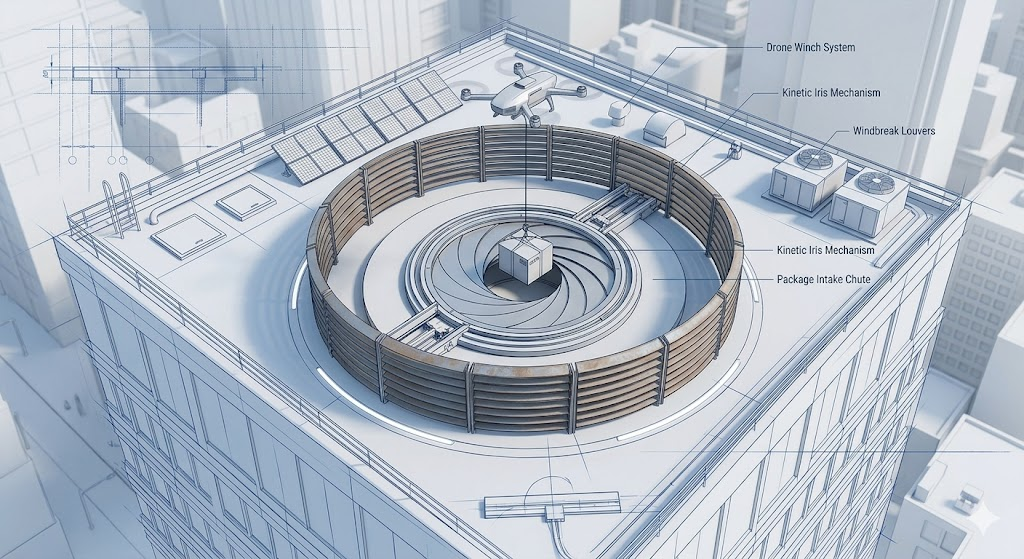
\includegraphics[width=\linewidth]{new-building-rooftop.png}
        \caption{New-construction Rooftop Flight Deck with wind-break louvers and catchment funnel.}
        \label{fig:rooftop}
    \end{subfigure}
    \hfill
    \begin{subfigure}{0.48\linewidth}
        \centering
        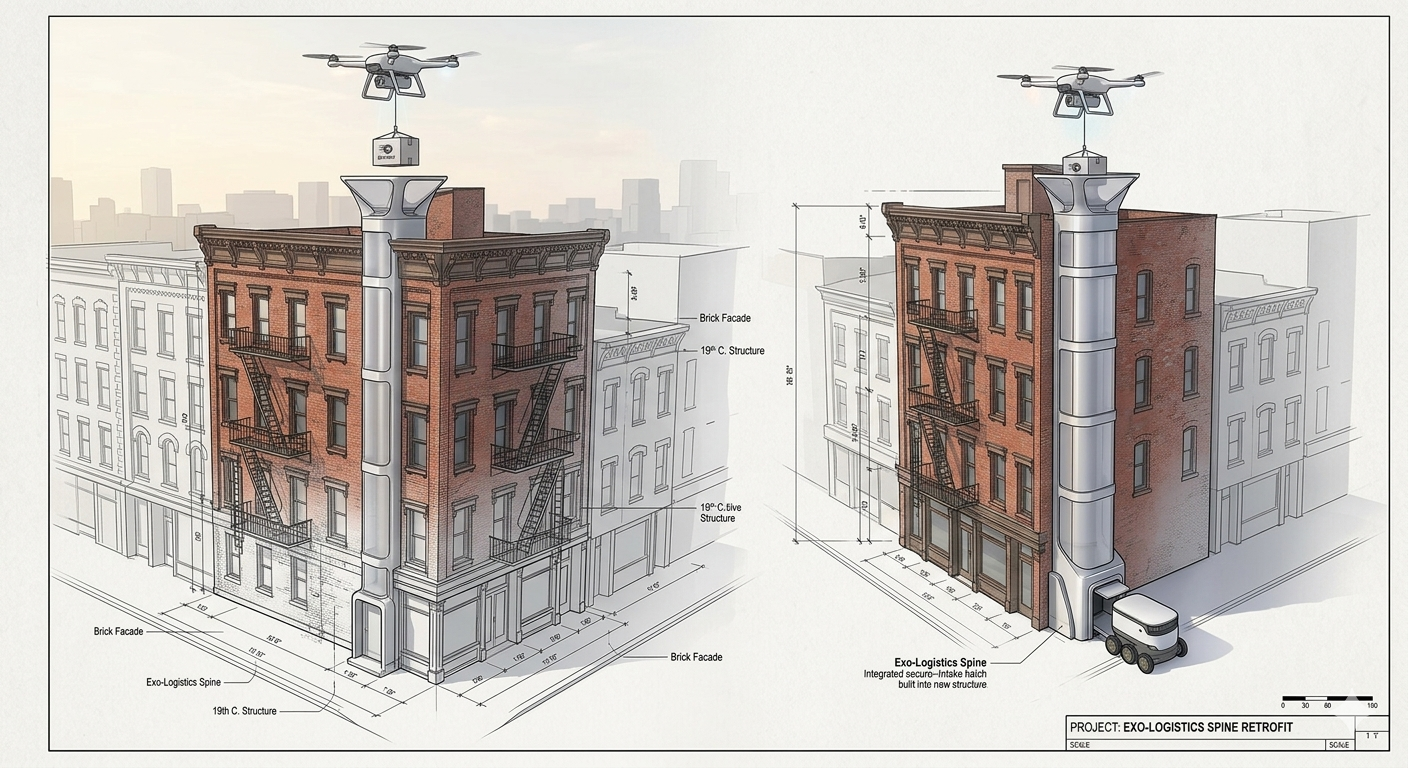
\includegraphics[width=\linewidth]{retrofit-pipe-desing-outside.png}
        \caption{Historic-retrofit Exo-Logistics Spine clipped to the facade.}
        \label{fig:spine-outside}
    \end{subfigure}
    \caption{Twin-track proposed solution: a vertically integrated rooftop core for new builds and a modular external spine for protected buildings.}
    \label{fig:twin-track}
\end{figure}

The innovation aspect is not any single mechanism but the
\emph{system-level} integration: the building itself becomes the
delivery infrastructure, multi-modal fleets are abstracted behind a
single API gateway, and the bulk of the parcel transport is
intentionally \emph{passive}---gravity chutes, motorized rollers, and
mechanical diverters---to keep cost, energy, and failure rates low.

\section{Breakthrough Technologies Required}
\label{sec:breakthroughs}

Delivering this twin-track system at scale requires advances in seven
specific technology areas:

\begin{description}[leftmargin=1.4cm,style=nextline]
    \item[Kinetic Weather-Sealing Mechanisms.] High-speed automated
    apertures---the ``Kinetic Iris Hatch''---that open and close in
    seconds to admit a parcel drop while maintaining 100\% climate
    isolation during severe weather.
    \item[Pneumatic Deceleration Systems.] Calculated internal air
    pressure inside the Exo-Logistics Spine to safely slow a
    free-falling package without active braking or parachutes.
    \item[Precision Dual-Claw Handover Robotics.] A choreographed pair
    of robotic claws---one in the micro-vestibule, one inside the
    elevator car---that hand a payload off without dropping it.
    \item[Parametric Wind-Shear Deflection.] Curved louver geometries
    and architectural materials that break up rooftop wind gusts and
    mitigate drone rotor downwash to keep the drone stable during the
    winch drop.
    \item[Intelligent, Self-Contained Elevator Chassis.] A vertical
    transport car for the retrofit tube that carries its own power,
    computing, and articulated arm, removing the need to install
    sorting hardware on every floor of an old building.
    \item[Integrated Building API and Fleet Gateway.] A unified
    ``Central Cloud'' that lets third-party fleets (e.g.~Google Wing,
    Yandex Rover) talk securely to the Building Automation System for
    real-time docking and hatch synchronization.
\end{description}

% =====================================================================
%  CHAPTER 3 - TEAM & INNOVATIVE PRODUCT
% =====================================================================
\chapter{Team and Innovative Product Development}
\label{ch:team-product}

\section{The Team and Capabilities}
\label{sec:team}

The Cargo-to-Door team combines systems engineering, mechanical and
robotic design, software-cloud orchestration, civil and architectural
integration, and regulatory expertise---six interlocking capabilities
that mirror the six engineering layers of the product itself
(Table~\ref{tab:team}).

\begin{table}[H]
\centering
\caption{Team roles and the capabilities each role brings to the project.}
\label{tab:team}
\small
\begin{tabularx}{\linewidth}{L{4.5cm} X}
\toprule
\textbf{Role} & \textbf{Capability brought} \\
\midrule
Principal Investigator     & Systems engineering, autonomous vehicles \\
Mechanical Lead            & Aerodynamic structures, pneumatic systems \\
Controls \& Robotics       & Drone control, robotic manipulation \\
Software \& Cloud          & Fleet orchestration, edge computing \\
Architecture \& Civil      & High-rise integration, historic-preservation retrofits \\
Business \& Regulatory     & Go-to-market, FAA / municipal liaison \\
\bottomrule
\end{tabularx}
\end{table}

\section{Requirements Definition and Analysis}
\label{sec:requirements}

Because the new-build and retrofit tracks share software but differ
physically, requirements are partitioned into two parallel sets.

\subsection{New Construction Requirements}
\label{ssec:req-new}

\paragraph{Functional requirements.}
\begin{itemize}
    \item \textbf{Aerial Intake Mechanism.} The system must feature a
    weather-sealed rooftop catchment funnel that opens to receive
    winch-dropped cargo from hovering drones without requiring them to
    land.
    \item \textbf{Internal Transport.} Received packages must move
    autonomously from the roof to the central vertical shaft using
    angled gravity chutes and motorized roller conveyors.
    \item \textbf{Automated Sorting.} Packages must be sorted and
    routed into waiting smart dumbwaiters via simple mechanical
    diverter flaps.
    \item \textbf{Floor-Level Distribution.} The smart dumbwaiter must
    deposit the package into a secure, integrated receiving locker in
    the hallway of the recipient's floor.
    \item \textbf{Micro-Rover Extraction.} The ground-floor
    micro-vestibule must use a ceiling-mounted robotic arm to extract
    cargo from autonomous sidewalk delivery robots and place it onto
    the internal conveyor network.
\end{itemize}

\paragraph{Non-functional requirements.}
\begin{itemize}
    \item \textbf{Aerodynamics \& Wind Mitigation.} Parametric, curved
    rooftop louvers must manage wind shear and drone rotor downwash so
    the drone remains stable while hovering.
    \item \textbf{Acoustic Isolation.} The centralized shaft must
    isolate high-frequency drone noise and conveyor sounds from
    residential living areas.
    \item \textbf{Maintainability \& Cost.} Primary sorting mechanics
    must prioritize passive systems (gravity and momentum) over complex
    robotics, minimizing maintenance, breakdowns, and energy use.
    \item \textbf{Security.} Access to the internal logistics core
    must be restricted; residents access only their own locker via
    digital app authentication.
    \item \textbf{Throughput Scalability.} The network must handle a
    high volume of concurrent deliveries without bottlenecking at the
    rooftop funnel during peak hours.
\end{itemize}

\subsection{Historic Retrofit Requirements}
\label{ssec:req-retrofit}

\paragraph{Functional requirements.}
\begin{itemize}
    \item \textbf{Modular Exterior Hub.} The system must provide an
    exterior-mounted Exo-Logistics Spine with a top-mounted kinetic
    weather hatch for aerial drone drops.
    \item \textbf{Intelligent Vertical Transit.} A mobile, intelligent
    elevator car must travel inside the spine to transport packages
    vertically.
    \item \textbf{Articulated Floor Delivery.} The elevator car must
    carry an internal robotic arm that reaches through a retrofitted
    window and places packages on a specific indoor resident shelf.
    \item \textbf{Dual-Claw Handover.} The ground-level intake must
    feature a dedicated robotic claw that extracts cargo from sidewalk
    micro-rovers and physically hands it to a second robotic claw
    inside the waiting elevator car.
    \item \textbf{Precision Alignment.} The mobile elevator car must
    mechanically align with the designated floor's retrofitted window
    opening before opening its hatch.
\end{itemize}

\paragraph{Non-functional requirements.}
\begin{itemize}
    \item \textbf{Modularity \& Structural Load.} The external tube
    must be lightweight, prefabricated, and modular, attachable to
    older masonry without violating historic load limits.
    \item \textbf{Weather \& Climate Resistance.} The kinetic hatches
    and tube casing must maintain a 100\% watertight environment in
    severe rain, snow, or freezing conditions.
    \item \textbf{Kinematic Precision.} Handover between ground claw,
    elevator car, and floor arm must be mechanically precise enough to
    prevent any drop outside the building.
    \item \textbf{Energy Efficiency.} The elevator car and arms must
    use optimized low-draw power systems compatible with the dated
    electrical grids common to historic buildings.
    \item \textbf{Aesthetic Integration.} The spine must present a
    clean high-tech industrial design that contrasts intentionally
    with 19th-century brick or stone facades while complying with
    urban-planning aesthetic codes.
\end{itemize}

\section{High-Level System Architecture}
\label{sec:architecture}

Cargo-to-Door is organized as five horizontal layers that span the
sky-to-resident path. Figure~\ref{fig:arch} renders the layer stack and
the principal data flows between them.

\begin{figure}[H]
\centering
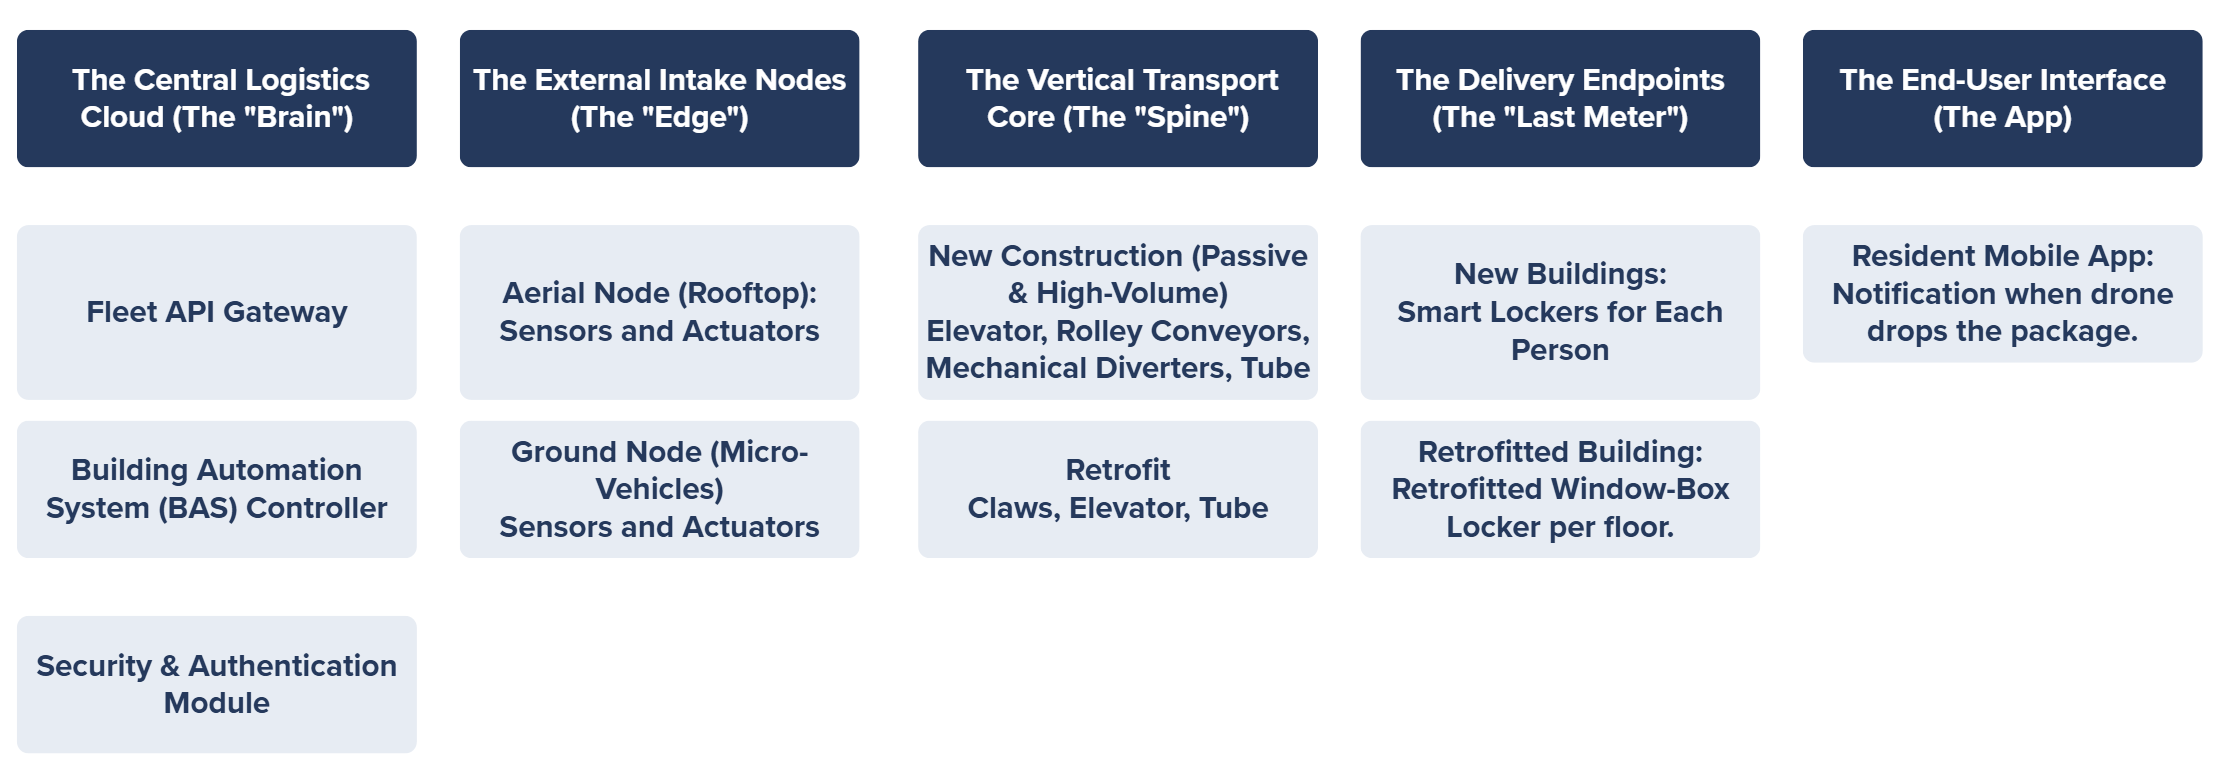
\includegraphics[width=\linewidth]{high-level-system-architecture.png}
\caption{Cargo-to-Door five-layer system architecture, from Central Cloud down to the resident's app.}
\label{fig:arch}
\end{figure}

\paragraph{Layer 1 -- The Central Logistics Cloud (``Brain'').}
A multi-tenant cloud platform that exposes a Fleet API Gateway to
third-party drone and rover operators, a Building Automation System
(BAS) Controller that talks to each building's actuators and sensors,
and a Security \& Authentication Module that issues per-delivery
credentials.

\paragraph{Layer 2 -- External Intake Nodes (``Edge'').}
Two physical entry points per building: an aerial rooftop node (kinetic
hatch, funnel, wind-break louvers, sensors, actuators) and a
ground-level node (kinetic docking hatch and robotic arm for micro
rovers). Each node runs edge logic for fast handshakes with the
incoming vehicle.

\paragraph{Layer 3 -- Vertical Transport Core (``Spine'').}
For new construction, this is the internal sorting shaft with elevator
modules, roller conveyors, mechanical diverters, and gravity chutes.
For retrofits, it is the external Exo-Spine tube containing the
intelligent elevator car and dual-claw handovers.

\paragraph{Layer 4 -- Delivery Endpoints (``Last Meter'').}
In new buildings, hallway-integrated smart lockers, one compartment per
delivery, with sliding logistics-core access. In retrofits, a single
window-box locker per floor served by the mobile elevator car's robotic
arm.

\paragraph{Layer 5 -- End-User Interface.}
A resident mobile application that issues push notifications
(``Package received: Unit~4C, Compartment~L16''), handles authentication
at the locker screen, and surfaces real-time delivery tracking.

\section{Design, Implementation, and Testing}
\label{sec:design}

This section walks through the major sub-systems---from the rooftop
down to the resident's hallway, and from the historic-building facade
down to its window-box locker---and then summarizes the implementation
and testing strategy.

\subsection{Embedded System Overview (New Construction)}
\label{ssec:design-new-overview}

The end-to-end vertical flow of the Embedded Residential Cargo System
for new construction is captured in a 1:100-scale 2D architectural
section (Figure~\ref{fig:new-overview}). The logistics path starts at
the roof drone platform, travels through the embedded cargo shaft, and
terminates at built-in smart mailboxes on the residential levels. The
same shaft network supports bidirectional flow by integrating with the
Ground Floor AGV Port and a built-in AGV Hub. At the top node, the
roof-integrated drone port provides a secure direct entry to the shaft
through a hinged cover mechanism shown in the open position. At the
delivery endpoint, cargo is handed to the apartment entryway through an
in-wall delivery cabinet via a flush-mount main facade access panel.

\begin{figure}[H]
    \centering
    \includegraphics[width=0.90\linewidth]{new-building-overview.png}
    \caption{1:100 2D system overview of the embedded new-construction cargo flow, from roof drone platform to in-wall apartment delivery cabinets, with integrated AGV ground interface.}
    \label{fig:new-overview}
\end{figure}

\subsection{Rooftop Flight Deck}
\label{ssec:design-rooftop}

The Flight Deck is a stable delivery zone framed by perforated
wind-break louvers that tame rooftop turbulence and shape an
aerodynamic catchment funnel sized for off-center hover drops
(Figure~\ref{fig:design-rooftop}). The drone executes a
\emph{hover-winch protocol}: it holds altitude $Z$ above the funnel
mouth, lowers the parcel on a tether, releases, and departs without
landing. Secure storage lockers on the deck hold high-value or
oversized parcels awaiting retrieval by building staff.

\begin{figure}[H]
    \centering
    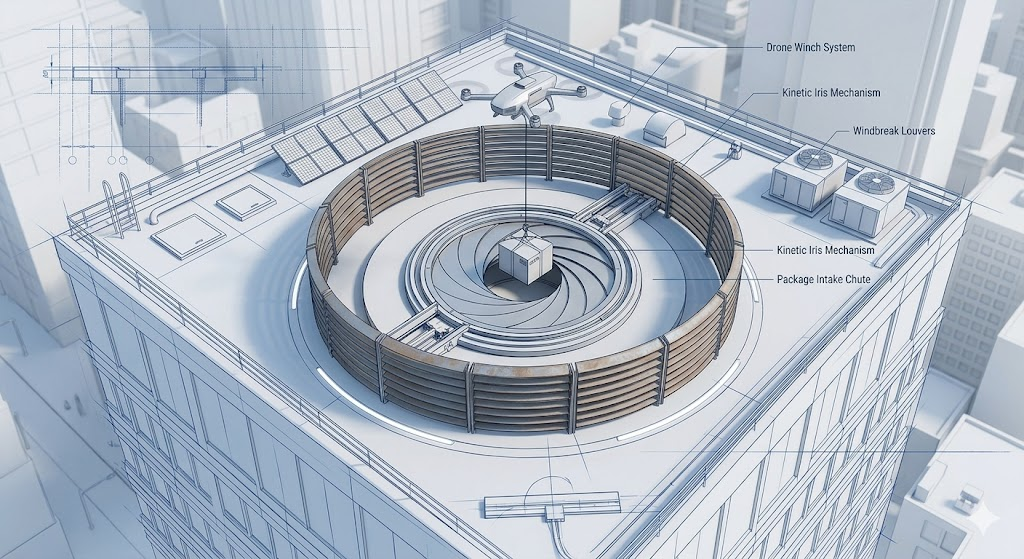
\includegraphics[width=0.85\linewidth]{new-building-rooftop.png}
    \caption{Rooftop Flight Deck with wind-break louvers, catchment funnel, and rooftop secure storage lockers.}
    \label{fig:design-rooftop}
\end{figure}

\subsection{Drop Funnel and S-Trap}
\label{ssec:design-funnel}

Below the funnel mouth the parcel enters a dry interior zone that opens
onto the autonomous internal sorting shaft and the first roller
conveyor (Figure~\ref{fig:design-funnel}). A passive \emph{S-Trap}---a
drainage geometry borrowed from plumbing---blocks wind-driven rain from
following the parcel down the shaft, without any active actuator.

\begin{figure}[H]
    \centering
    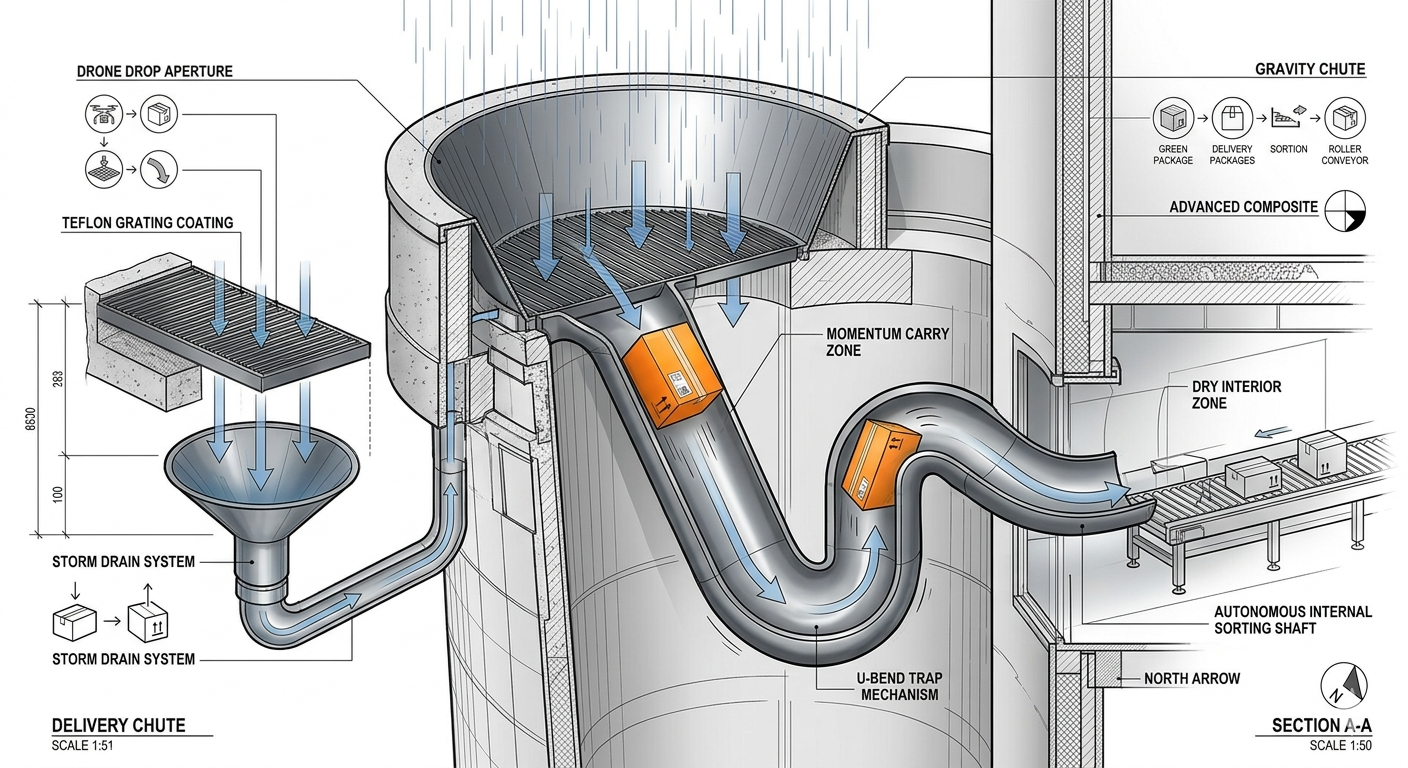
\includegraphics[width=0.75\linewidth]{new-building-get-cargo.png}
    \caption{Catchment funnel and S-Trap drop transition into the internal sorting shaft.}
    \label{fig:design-funnel}
\end{figure}

\subsection{Internal Sorting Core}
\label{ssec:design-sorting}

The internal sorting core (Figure~\ref{fig:design-sorting}) is a
deliberately passive logistics network: a stainless-steel gravity chute
moves parcels from the rooftop core toward floor-level receiving bays,
a motorized roller conveyor combined with diverter flaps routes each
parcel to its destination column, and a smart dumbwaiter---an
open-front car in a dedicated shaft---lifts or lowers the parcel to the
resident's floor.

\begin{figure}[H]
    \centering
    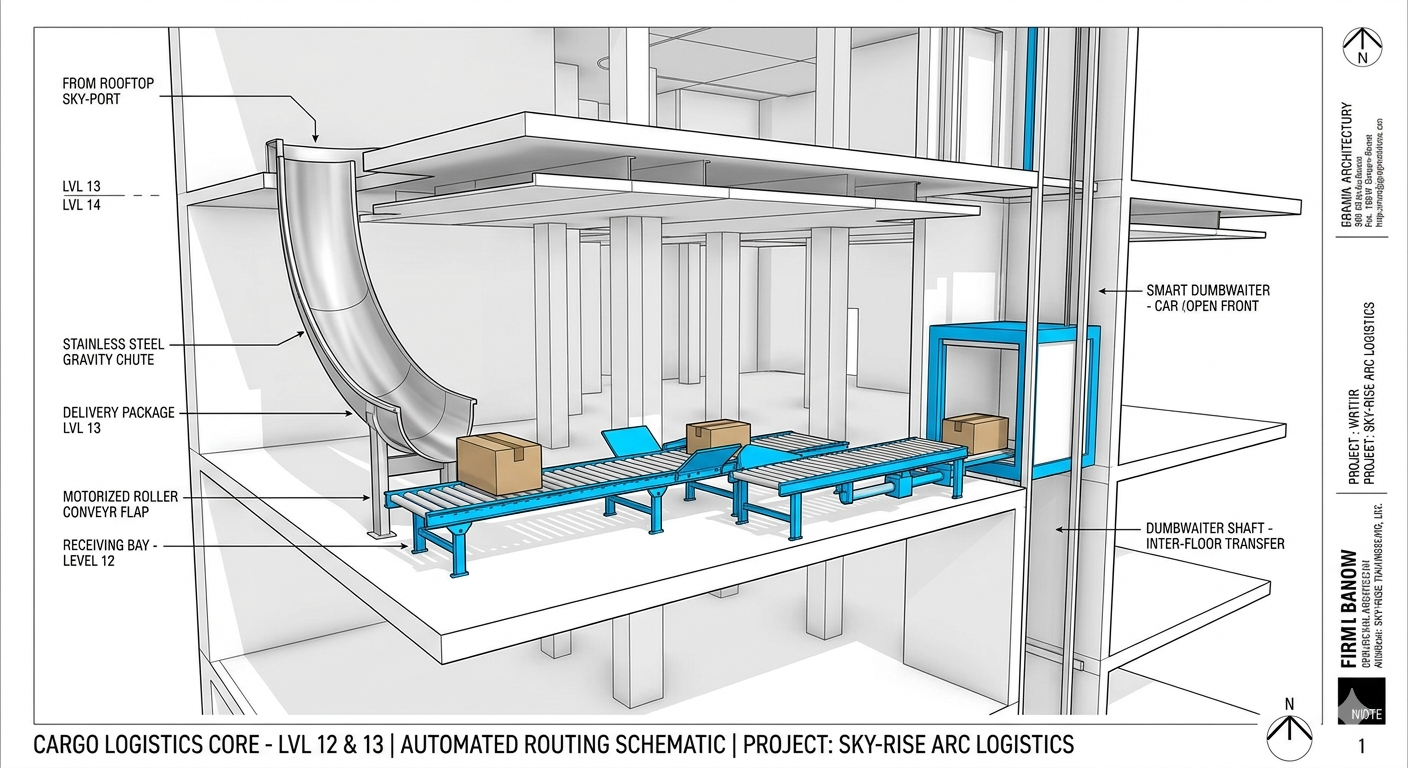
\includegraphics[width=0.80\linewidth]{new-building-seperator.png}
    \caption{Internal sorting core: gravity chute, motorized rollers, and mechanical diverter flaps.}
    \label{fig:design-sorting}
\end{figure}

\subsection{Resident Smart-Locker Array}
\label{ssec:design-lockers}

The hallway endpoint is an integrated smart-locker array built into
the apartment-floor wall behind a wood-and-glass facade with embedded
tech inserts (Figure~\ref{fig:design-lockers}). A sliding secure
logistics core behind the lockers connects directly to the vertical
shaft. Once a parcel is placed, the resident receives a push
notification (``Package received: Unit~4C, Compartment~L16''),
authenticates at the screen, and the matching compartment opens.

\begin{figure}[H]
    \centering
    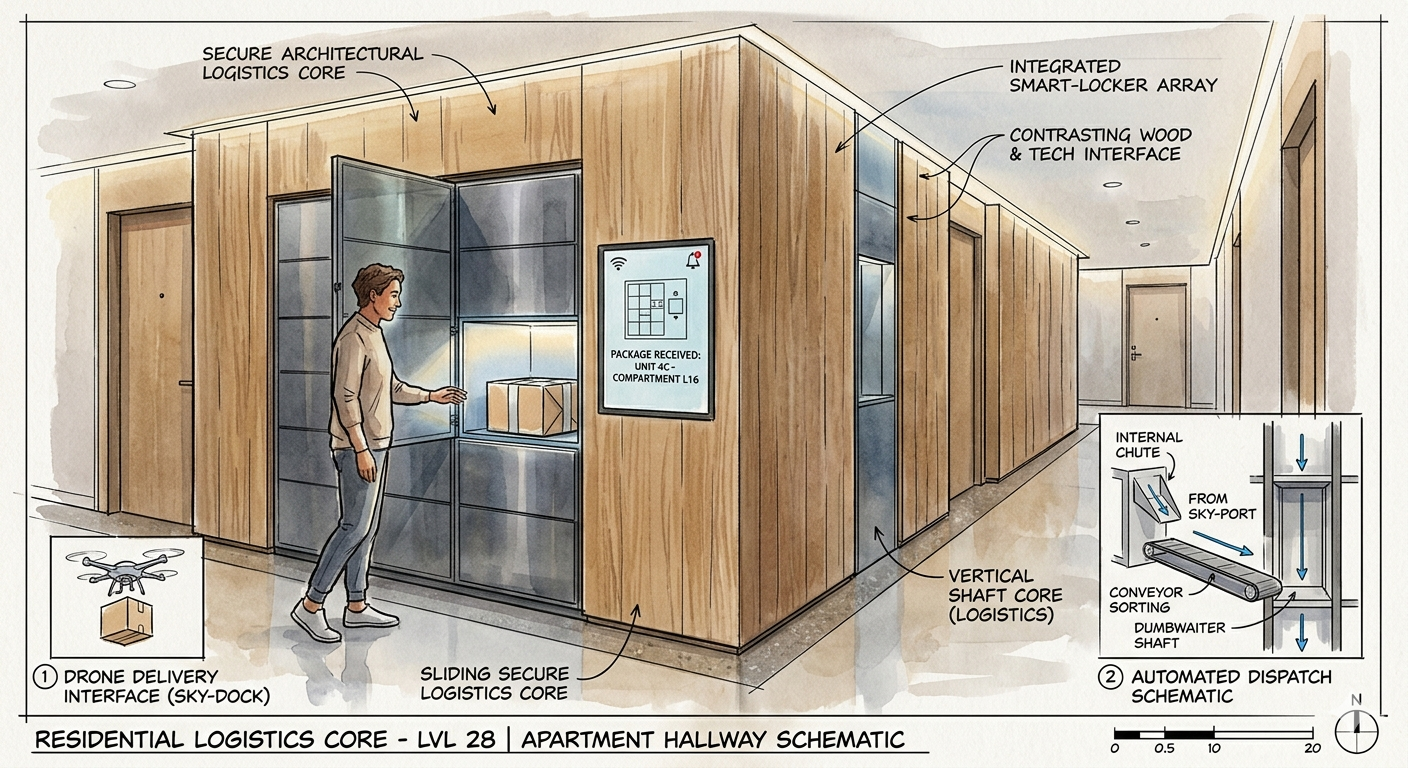
\includegraphics[width=0.80\linewidth]{new-building-smart-locker.png}
    \caption{Hallway-integrated smart-locker array with authentication screen and sliding logistics core behind the wall.}
    \label{fig:design-lockers}
\end{figure}

\subsection{Ground-Level Micro-Rover Interface}
\label{ssec:design-rover}

Sidewalk micro-rovers approach a segregated micro-logistics lane and
dock at a kinetic hatch in the facade
(Figure~\ref{fig:design-rover}\subref{fig:rover-outside}). Inside the
vestibule, a ceiling-mounted precision robotic arm lifts parcels off
the rover's open cargo bin and places them onto a motorized roller
conveyor that feeds the same internal sorting core used by aerial
deliveries (Figure~\ref{fig:design-rover}\subref{fig:rover-inside}).

\begin{figure}[H]
    \centering
    \begin{subfigure}{0.48\linewidth}
        \centering
        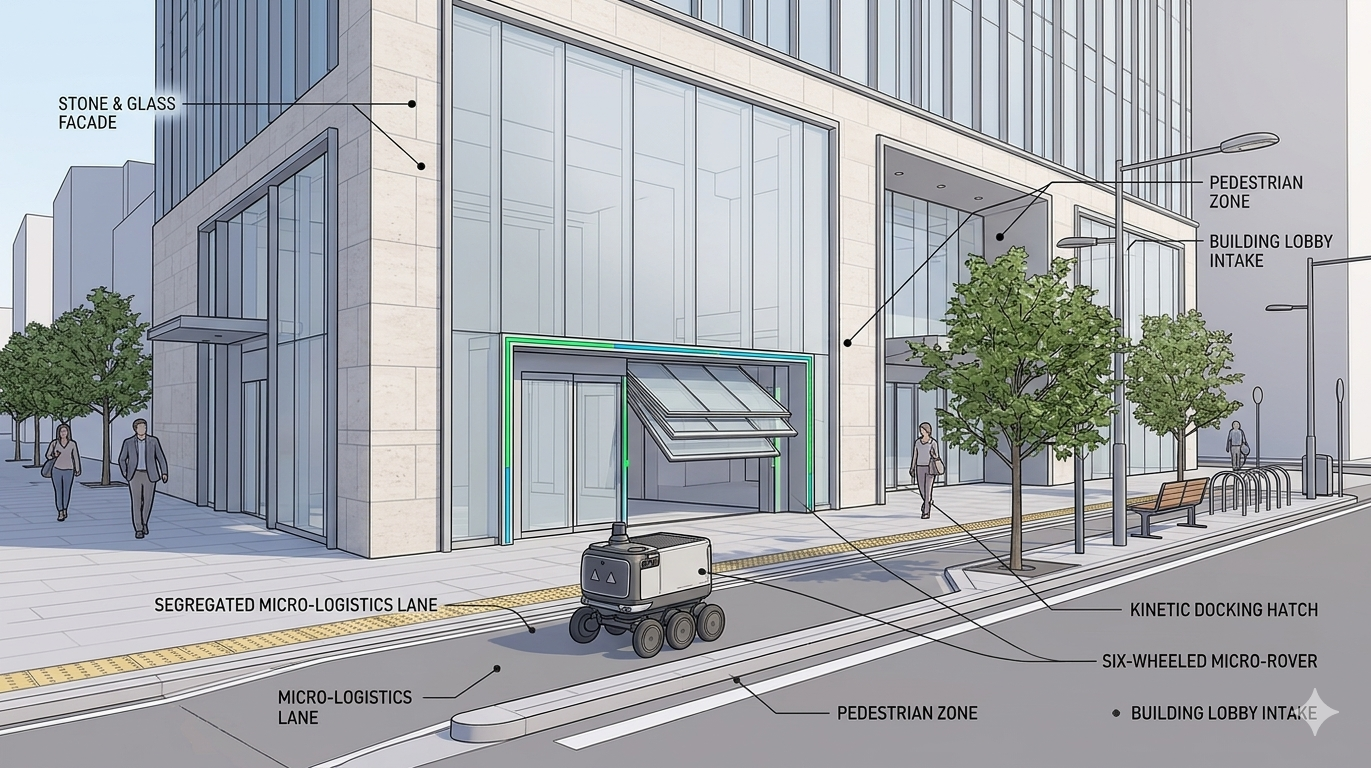
\includegraphics[width=\linewidth]{new-building-rover.png}
        \caption{Sidewalk rover approaching the kinetic docking hatch.}
        \label{fig:rover-outside}
    \end{subfigure}
    \hfill
    \begin{subfigure}{0.48\linewidth}
        \centering
        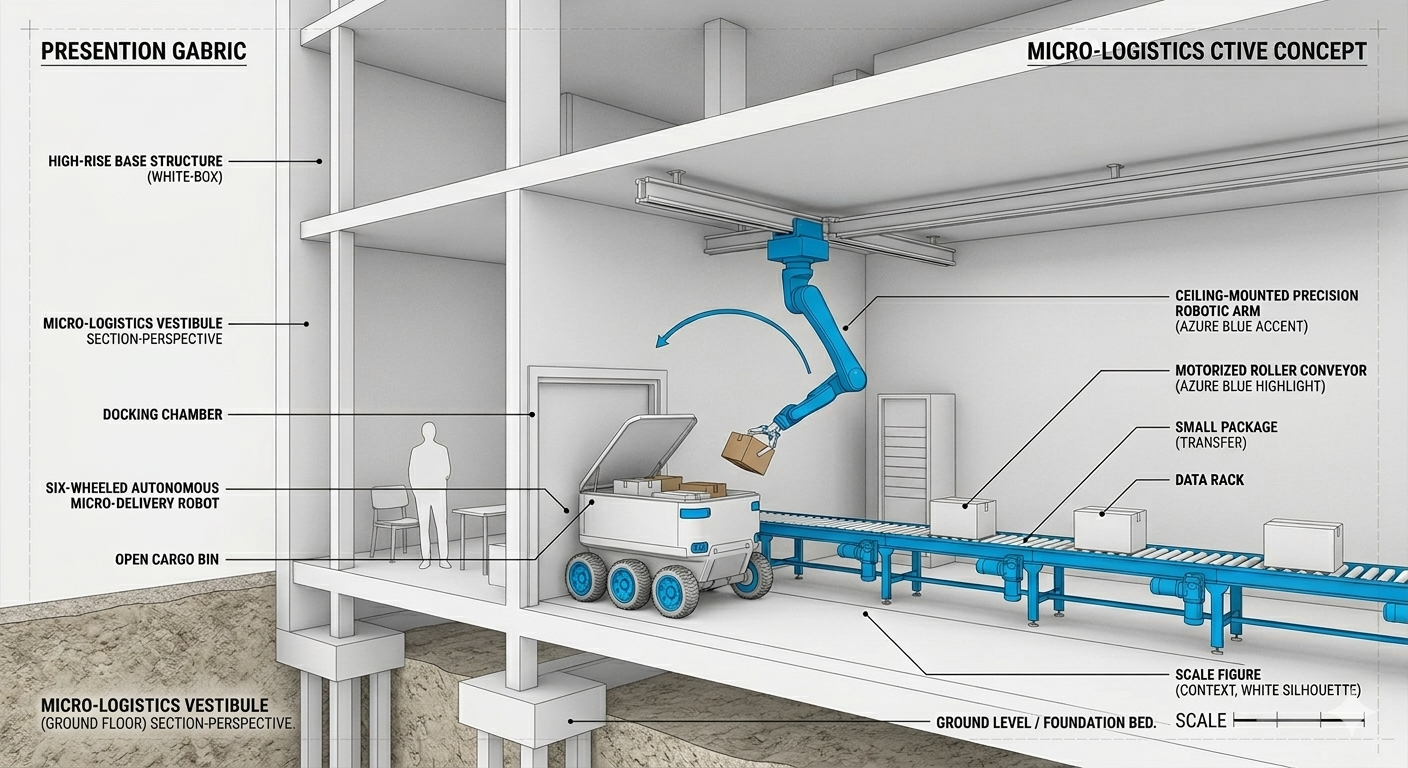
\includegraphics[width=\linewidth]{new-building-rover-get.png}
        \caption{Ceiling-mounted precision robotic arm extracts parcel inside the vestibule.}
        \label{fig:rover-inside}
    \end{subfigure}
    \caption{Ground-level micro-rover interface for new-construction buildings.}
    \label{fig:design-rover}
\end{figure}

\subsection{Retrofit Exo-Logistics Spine}
\label{ssec:design-spine}

The modular retrofit delivery system for existing multi-unit buildings
combines an adaptive logistics full-scale facade elevator with an
integrated apartment box solution (Figure~\ref{fig:retrofit-overview}).
The 2D overview shows the autonomous ground AGV docking station, the
automated roof drone platform, the facade-elevator retrofit that
requires no interior renovation, and the direct-to-unit transfer path
to personalized apartment delivery boxes. Vertical movement is
performed by an elevator rail attached to the existing facade. The
platform includes an automatic hatch and a package transfer arm that
routes cargo into the vertical spine, while an add-on transfer
mechanism with a package pusher safely completes the handoff from the
exterior rail to the apartment interior.

\begin{figure}[H]
    \centering
    \includegraphics[width=0.90\linewidth]{retrofit-overview.png}
    \caption{2D retrofit system overview: AGV docking, roof drone intake, facade elevator rail, vertical spine, and direct-to-unit apartment box transfer.}
    \label{fig:retrofit-overview}
\end{figure}

For protected buildings, the Exo-Logistics Spine is a prefabricated
vertical tube clipped to the facade
(Figure~\ref{fig:spine-exterior}). Internally, a self-contained smart
elevator car carries the parcel to the addressed floor, mechanically
aligns with a retrofitted window opening, and an articulated arm
reaches through to place the parcel directly on the resident's indoor
shelf (Figure~\ref{fig:spine-interior}). Because the spine carries its
own power and computing, it requires neither per-floor sorting hardware
nor invasive modifications to the historic interior.

\begin{figure}[H]
    \centering
    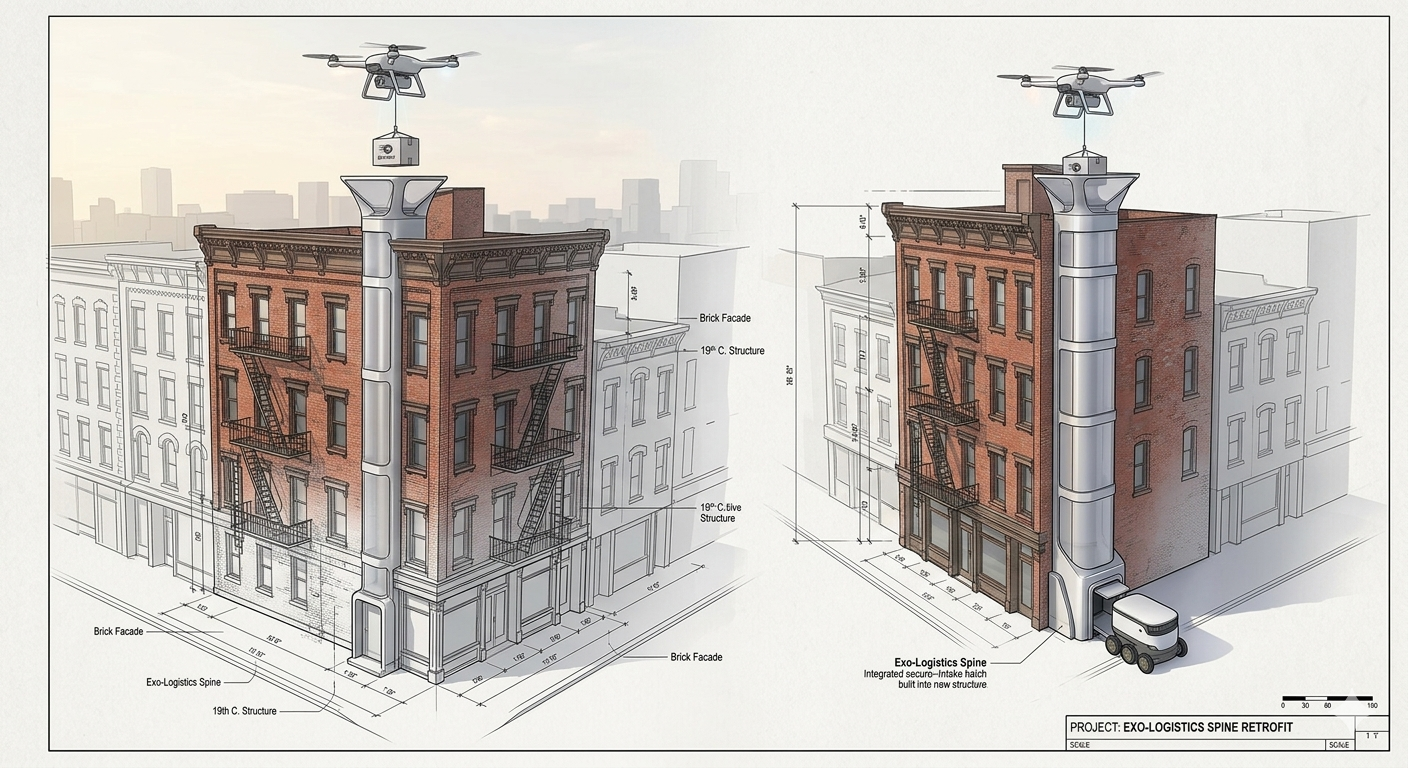
\includegraphics[width=0.78\linewidth]{retrofit-pipe-desing-outside.png}
    \caption{Exo-Logistics Spine clipped to a historic facade, with kinetic weather hatch at the top.}
    \label{fig:spine-exterior}
\end{figure}

\begin{figure}[H]
    \centering
    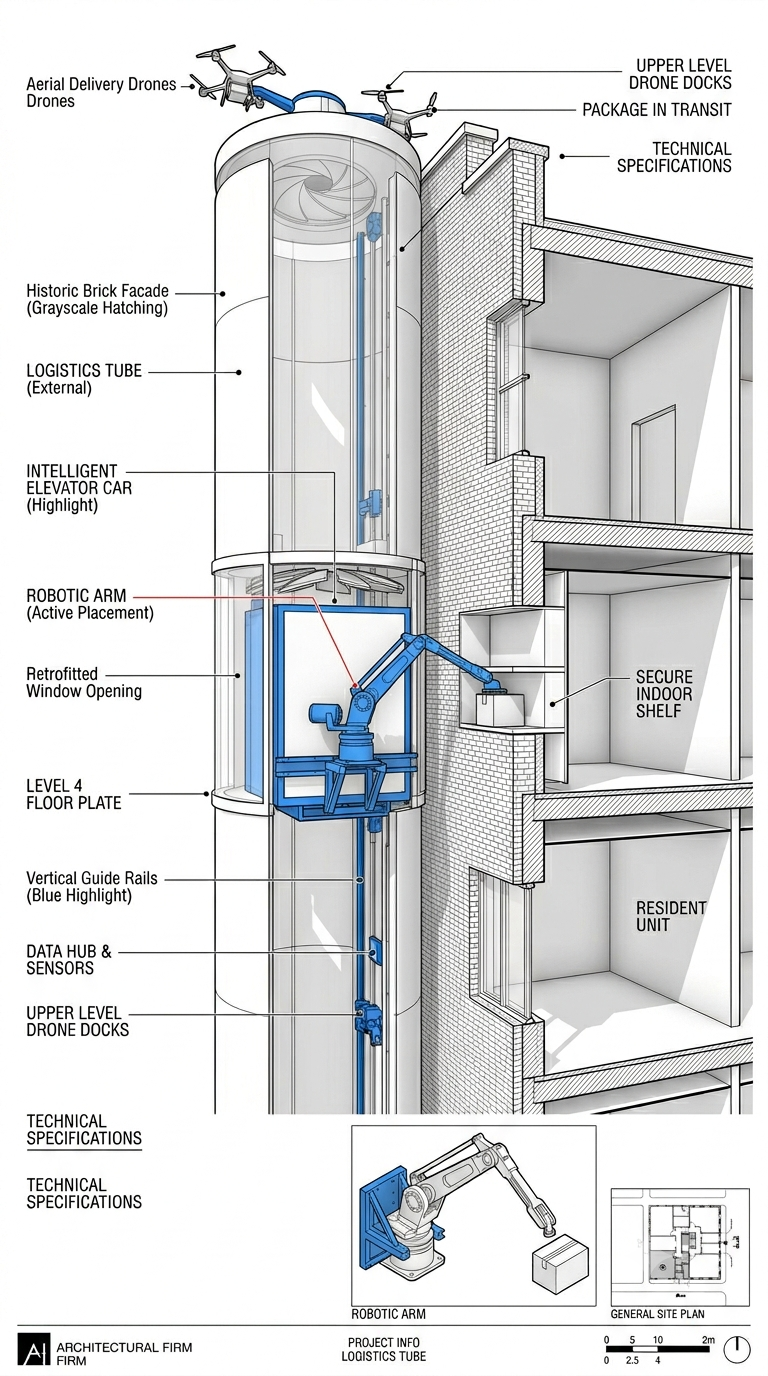
\includegraphics[width=0.78\linewidth]{retrofit-tube-design.png}
    \caption{Smart elevator car inside the Exo-Spine, robotic arm reaching through a retrofitted window-box locker onto a resident's shelf.}
    \label{fig:spine-interior}
\end{figure}

\subsection{Retrofit Rover Handover}
\label{ssec:design-retrofit-rover}

Retrofits share the multi-modal ground intake. A dedicated robotic
claw extracts a parcel from the sidewalk micro-rover and performs a
precision dual-claw handover with a second claw inside the waiting
elevator car at the base of the Exo-Spine
(Figure~\ref{fig:design-retrofit-rover}).

\begin{figure}[H]
    \centering
    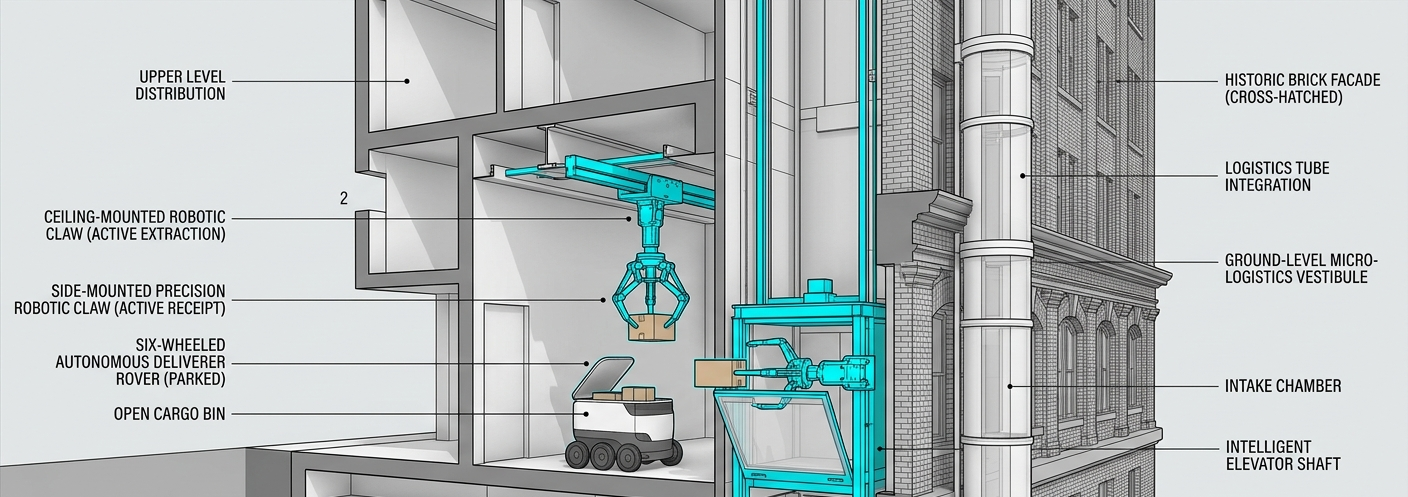
\includegraphics[width=0.78\linewidth]{retrofit-tube-design-rover.png}
    \caption{Retrofit ground intake: dual-claw handover from sidewalk rover into the Exo-Spine elevator car.}
    \label{fig:design-retrofit-rover}
\end{figure}

\subsection{Implementation and Testing}
\label{ssec:impl-test}

\paragraph{Key Performance Indicators.}
The system's KPIs span mechanical/logistics and
environmental/architectural categories.

\begin{itemize}
    \item \textbf{Package Throughput Rate.} Packages successfully
    transferred from the aerial funnel or ground vestibule to the
    destination locker per hour. \emph{Target:} $> 30$
    packages/hour/shaft.
    \item \textbf{Handover Success Rate.} Percentage of flawless
    mechanical transfers (drone-to-funnel, rover-to-claw,
    claw-to-elevator) without a drop or jam. \emph{Target:} 99.99\%.
    \item \textbf{Mean Time Between Failures (MTBF).} Operational time
    between breakdowns of active components (kinetic hatch, robotic
    extraction claw).
    \item \textbf{Acoustic Leakage.} Maximum noise inside the nearest
    residential unit during a drone drop or dumbwaiter cycle.
    \emph{Target:} $< 35$\,dB (library-ambient).
    \item \textbf{Weather Ingress Limit.} Water bypassing the kinetic
    hatch under simulated heavy rain. \emph{Target:} 0.0\,L.
    \item \textbf{Wind Deflection Efficiency.} Reduction in wind shear
    inside the rooftop funnel vs. the open exterior, measured by
    anemometer. \emph{Target:} $> 80$\% reduction.
\end{itemize}

\paragraph{Testing strategy.}
The testing strategy is layered, moving from individual components up
through environmental stress and user acceptance:

\begin{enumerate}
    \item \textbf{Component Testing (Lab \& Wind Tunnel).} Robotic
    claws and kinetic hatches are cycled through 100{,}000 continuous
    open/close operations to characterize motor fatigue and hinge
    durability. Parcels of varying weight and material (cardboard,
    plastic mailers) are dropped through the tube to verify
    jam-resistance.
    \item \textbf{Sub-System Integration Testing (the ``Handshake'').}
    \emph{Aerial handshake:} a drone hovering over the funnel
    measures the latency of the authentication protocol---does the
    iris hatch open fast enough, and close before the drone leaves?
    \emph{Dual-claw handover:} the ground claw transfers a dummy
    parcel to the elevator-car claw 500 times, with misalignments
    measured in millimeters.
    \item \textbf{Environmental Stress Testing.} A monsoon test sprays
    high-pressure water directly onto closed kinetic hatches while
    deliveries continue. A thermal-freeze test operates the
    Exo-Spine elevator and kinetic switchers at sub-zero temperatures
    to confirm lubricants and pneumatic seals survive.
    \item \textbf{User Acceptance Testing (UAT).} Beta residents are
    timed end-to-end from notification scan to locker retrieval, and
    sound engineers measure in-apartment decibel spikes during a
    simulated peak delivery hour.
\end{enumerate}

% =====================================================================
%  CHAPTER 4 - ROADMAP
% =====================================================================
\chapter{Roadmap and Project Plan}
\label{ch:roadmap}

The Cargo-to-Door pilot is planned as a 24-month, five-phase program
that moves from simulation through component prototyping, an
integrated test rig, regulatory pilot preparation, and a real-world
pilot deployment in one new-build tower and one retrofit block.

\section{Phased Plan}
\label{sec:phases}

\begin{table}[H]
\centering
\caption{Five-phase 24-month plan with exit gates.}
\label{tab:phases}
\small
\begin{tabularx}{\linewidth}{L{4.4cm} L{1.6cm} X L{4.0cm}}
\toprule
\textbf{Phase} & \textbf{Months} & \textbf{Focus} & \textbf{Exit gate} \\
\midrule
P1 -- Feasibility \& Simulation              & 1--3   & Validate airflow, routing logic, structural constraints, and safety assumptions. & Digital twin + initial safety case completed. \\
P2 -- Component Prototyping                  & 4--8   & Build and test key modules: funnel, hatch, chute, rover dock, locker interface. & Bench-test sign-off. \\
P3 -- Integrated Test Rig                    & 9--14  & Combine rooftop intake, vertical transport, smart locker, and app workflow in a controlled mockup. & End-to-end package delivery demonstrated. \\
P4 -- Building \& Regulatory Pilot Prep      & 15--18 & Prepare code compliance, fire safety, drone operation approvals, and stakeholder agreements. & Pilot building selected and permits submitted. \\
P5 -- Real-World Pilot Deployment            & 19--24 & One new-build tower + one retrofit block.                                        & Operational pilot with real users and partner deliveries. \\
\bottomrule
\end{tabularx}
\end{table}

\section{Milestones, Deliverables, and Work Packages}
\label{sec:wps}

The phased plan is executed through seven work packages, each owned by
a lead capability and tied to a measurable success criterion
(Table~\ref{tab:wps}).

\begin{table}[H]
\centering
\caption{Work packages, deliverables, success measures, and target months.}
\label{tab:wps}
\small
\begin{tabularx}{\linewidth}{L{0.8cm} L{3.4cm} X X L{1.0cm}}
\toprule
\textbf{WP} & \textbf{Title} & \textbf{Key deliverables} & \textbf{Success measure} & \textbf{Month} \\
\midrule
WP1 & Rooftop Intake System          & Flight deck, wind-break louvers, catchment funnel, kinetic hatch         & Safe drone hover-drop without landing                & M8  \\
WP2 & Weatherproof Transfer System   & Sealed chute entry, moisture isolation                                   & Zero water ingress during rain testing               & M12 \\
WP3 & Internal Vertical Logistics Core & Sorting shaft, diverters, dumbwaiter / elevator module                 & Package routed to correct floor                      & M14 \\
WP4 & Resident Smart-Locker Interface & Floor-level lockers, access screen, app authentication                  & Resident retrieves package securely                  & M12 \\
WP5 & Ground Micro-Rover Interface   & Docking hatch, robotic arm, conveyor transfer                            & Rover-to-building handover succeeds                  & M16 \\
WP6 & Software \& Cloud Orchestration & Fleet API, routing engine, resident app, telemetry dashboard            & End-to-end delivery tracked digitally                & M20 \\
WP7 & Safety, Compliance \& Pilot Ops & Risk assessment, building-code review, drone approval, pilot plan       & Pilot-ready safety and approval package              & M24 \\
\bottomrule
\end{tabularx}
\end{table}

\section{Task Allocation and Timeline}
\label{sec:timeline}

Figure~\ref{fig:gantt} renders the 24-month timeline as a Gantt chart.
Each phase bar maps to the work packages active during that phase;
WP6 (software) and WP7 (safety) run across the full program in support
of the others.

\begin{figure}[H]
    \centering
    \includegraphics[width=\linewidth]{gantt-chart.png}
    \caption{24-month Cargo-to-Door Gantt chart. Phases P1--P5 are sequential; WP6 (software/cloud) and WP7 (safety/compliance) run as cross-cutting work packages.}
    \label{fig:gantt}
\end{figure}

% =====================================================================
%  CHAPTER 5 - COMMERCIALIZATION & BUSINESS MODEL
% =====================================================================
\chapter{Commercialization and Business Model}
\label{ch:business}

\section{Market Analysis}
\label{sec:market}

\paragraph{Target customers.}
The primary customers are \emph{residential developers, building
owners, and property management companies} who can purchase
Cargo-to-Door as a smart-building amenity. The end users are
\emph{residents of high-rise apartments} demanding secure, convenient
package delivery. Channel partners are \emph{drone delivery
companies, courier companies, e-commerce platforms, and sidewalk-rover
operators} that plug into the Cargo-to-Door API.

\paragraph{Beachhead market.}
The initial beachhead is \emph{premium high-rise residential buildings
and smart-city districts} where residents already expect
concierge-level services. Table~\ref{tab:market-fit} maps the principal
needs of this segment to Cargo-to-Door's product fit.

\begin{table}[H]
\centering
\caption{Needs of the beachhead market and Cargo-to-Door fit.}
\label{tab:market-fit}
\small
\begin{tabularx}{\linewidth}{L{4.5cm} X}
\toprule
\textbf{Need} & \textbf{Why Cargo-to-Door fits} \\
\midrule
High package volume               & Many residents per tower create dense, recurring delivery demand. \\
Security concerns                 & Reduces theft, failed deliveries, and lobby congestion. \\
Premium building positioning      & ``Logistics-ready building'' becomes a marketable differentiator. \\
Easier ROI justification          & Developers can capitalize the system as smart-building infrastructure. \\
Controlled environment            & Easier to pilot than city-wide deployment. \\
\bottomrule
\end{tabularx}
\end{table}

\paragraph{Market entry and growth.}
Cargo-to-Door enters the market through a small number of
\emph{lighthouse pilot buildings} in premium high-rise districts (one
new-build tower plus one retrofit block under WP7), then expands
horizontally to additional towers in the same district before
templating the integration for other developers and other cities.

\section{Business Model}
\label{sec:business-model}

Cargo-to-Door is a hardware-plus-software-plus-delivery-fees business
with five recurring or one-time revenue streams
(Table~\ref{tab:revenue}).

\begin{table}[H]
\centering
\caption{Revenue streams and payers.}
\label{tab:revenue}
\small
\begin{tabularx}{\linewidth}{L{4.8cm} L{4.6cm} X}
\toprule
\textbf{Revenue stream} & \textbf{Who pays} & \textbf{Description} \\
\midrule
Installation / integration fee     & Developer or building owner          & One-time fee for rooftop hub, vertical core, smart lockers, and building integration. \\
Monthly platform subscription      & Building owner / property manager    & Software orchestration, monitoring, authentication, maintenance dashboard. \\
Per-delivery transaction fee       & Logistics partners                   & Fee for each successful automated delivery routed through the system. \\
Maintenance \& service contract    & Building owner                       & Preventive maintenance, inspections, repairs, replacement parts. \\
Premium resident services          & Optional resident subscription       & Priority delivery, cold-chain locker, scheduled windows, high-security compartments. \\
\bottomrule
\end{tabularx}
\end{table}

\section{Competitor Analysis and Competitive Advantage}
\label{sec:competition}

Cargo-to-Door does not compete head-on with any single existing
solution; it instead \emph{connects} the gaps between them
(Table~\ref{tab:competition}).

\begin{table}[H]
\centering
\caption{Existing solutions and the gap Cargo-to-Door closes.}
\label{tab:competition}
\small
\begin{tabularx}{\linewidth}{L{4.0cm} L{4.0cm} X}
\toprule
\textbf{Existing solution} & \textbf{What it solves} & \textbf{Remaining gap} \\
\midrule
Drone delivery companies   & Fast aerial transport            & Cannot reliably deliver inside vertical buildings. \\
Sidewalk robots            & Low-cost local delivery          & Stop at building entrance or lobby. \\
Parcel lockers             & Secure pickup                    & Resident still travels to lobby or shared area. \\
In-building robots         & Interior delivery                & Depend on elevators; no exterior intake. \\
Pneumatic tube systems     & Internal automated transfer      & Require fixed infrastructure; lack drone/rover integration. \\
\bottomrule
\end{tabularx}
\end{table}

\paragraph{Our advantage.}
Cargo-to-Door connects the missing chain:
\[
\text{Drone / rover} \rightarrow \text{building intake} \rightarrow
\text{vertical transport} \rightarrow \text{resident floor} \rightarrow
\text{secure locker}.
\]

\paragraph{Competitive moat.}
\begin{itemize}
    \item Building-integrated physical infrastructure with high
    switching costs.
    \item Multi-modal intake supporting drones, rovers, and human
    couriers behind one API.
    \item Twin product lines covering both new-build and retrofit
    buildings.
    \item Weatherproof and secure end-to-end delivery path.
    \item Software layer connecting fleets, buildings, and residents.
\end{itemize}

\section{Budget, Pricing, and Monetization}
\label{sec:budget}

Pricing is structured so that the developer or building owner pays the
\emph{capital} cost (installation), the property manager pays the
\emph{operational} cost (monthly platform plus maintenance), the
logistics partners pay \emph{per delivery} (variable revenue that
scales with system utilization), and residents may optionally pay for
premium services (a high-margin upsell channel). This layered model
distributes risk across the parties that benefit from each layer of
value, accelerates payback for the developer through smart-building
positioning, and creates a recurring software-margin floor for the
operator. Quantitative pricing per market segment will be set during
WP7 based on observed pilot economics.

\section{Challenges and Business Risks}
\label{sec:risks}

The principal risks span regulatory, environmental, structural,
mechanical, social, financial, and integration domains
(Table~\ref{tab:risks}). Each is paired with a concrete mitigation
that has been baked into the system's design choices---most notably
the multi-modal intake (so the building remains useful even if aerial
delivery is regulated away) and the passive, gravity-driven core (so
mechanical failure modes are inherently bounded).

\begin{table}[H]
\centering
\caption{Top business and engineering risks and their mitigations.}
\label{tab:risks}
\small
\begin{tabularx}{\linewidth}{L{4.0cm} L{1.6cm} L{1.6cm} X}
\toprule
\textbf{Risk} & \textbf{Likelihood} & \textbf{Impact} & \textbf{Mitigation} \\
\midrule
Drone regulation delays              & High   & High   & Accept rovers and human couriers so the building infrastructure remains useful even if aerial delivery is delayed. \\
Weather limitations                  & Medium & High   & Weatherproof rooftop intake plus ground-level rover fallback during unsafe drone conditions. \\
Building code restrictions           & Medium & High   & Engage fire-safety, building-code, and elevator/shaft compliance experts from the early design phase. \\
Historic preservation rejection      & Medium & High   & Reversible, modular, low-impact Exo-Spine design with minimal facade penetration. \\
Mechanical reliability issues        & Medium & High   & Prefer passive gravity-based mechanisms and use telemetry-based predictive maintenance. \\
Resident acceptance concerns         & Medium & Medium & Reduce noise, protect privacy, use secure authentication, and communicate benefits clearly. \\
High installation cost               & High   & Medium & Start with premium high-rise buildings and prove ROI through a lighthouse pilot before scaling. \\
Logistics partner integration delays & Medium & Medium & Provide a standard API gateway and begin with one pilot logistics partner before expanding to multiple fleets. \\
\bottomrule
\end{tabularx}
\end{table}

% =====================================================================
%  APPENDIX
% =====================================================================
\appendix

\chapter{Pilot Success Criteria}
\label{app:pilot-kpis}

By the end of the 24-month pilot, the Cargo-to-Door system is required
to demonstrate the operational targets summarized in
Table~\ref{tab:pilot-targets}.

\begin{table}[H]
\centering
\caption{Pilot success criteria.}
\label{tab:pilot-targets}
\small
\begin{tabularx}{\linewidth}{L{4.5cm} X}
\toprule
\textbf{Category} & \textbf{Target} \\
\midrule
Delivery success         & $\geq 95$\% successful end-to-end deliveries in pilot conditions. \\
Handover reliability     & $\geq 99$\% successful mechanical handovers in controlled testing. \\
Package throughput       & 30+ packages/hour per shaft in peak simulation. \\
Resident retrieval time  & Under 60 seconds from notification to locker opening. \\
Weather protection       & No water ingress during simulated heavy rain. \\
Security                 & Only authenticated residents can access assigned compartments. \\
Operational readiness    & Maintenance issues detected through telemetry before failure. \\
\bottomrule
\end{tabularx}
\end{table}

% =====================================================================
%  BIBLIOGRAPHY
% =====================================================================
\begin{thebibliography}{9}

\bibitem{uav2022}
``Unmanned Aerial Vehicles for High-Density Residential Delivery,''
2022.

\bibitem{grid2023}
``Drone High-Rise Aerial Delivery with Vertical Grid Screening,''
2023.

\bibitem{slr2024}
``Drones in last-mile delivery: a systematic literature review from a
logistics management perspective,'' 2024.

\bibitem{integrated2025}
``Integrated Planning of Infrastructure and Drone Delivery Operations
with Multiple Cycles,'' 2025.

\bibitem{wind2025}
``Wind-Aware Service Provisioning Strategy for Multi-Package Drone
Delivery,'' 2025.

\end{thebibliography}

\end{document}
